\documentclass[conference, a4paper]{IEEEtran}
\IEEEoverridecommandlockouts
\usepackage[turkish]{babel}
\usepackage[utf8]{inputenc}
\usepackage[T1]{fontenc}
\usepackage[pdftex]{graphicx}
\usepackage{multirow}
\usepackage{cite}
\usepackage[cmex10]{amsmath}
\usepackage{siunitx}
\usepackage{array}
\usepackage[caption=false,lofdepth,lotdepth]{subfig}
\usepackage{booktabs}
\usepackage{float}
\usepackage{url}
\usepackage{acronym}

\setlength{\textfloatsep}{5pt}

\AtBeginDocument{%
	\renewcommand\tablename{TABLO}
}

\AtBeginDocument{%
	\renewcommand\abstractname{Abstract}
}

\graphicspath{{../results/}{../results/plots/}}

\begin{document}
\shorthandoff{=}

\title{NPM Tedarik Zincirinde Topolojik Risk Analizi ve Kritiklik Haritalaması\\
 Topological Risk Analysis and Criticality Mapping in the NPM Supply Chain}

\author{\IEEEauthorblockN{Yusuf Talha ARABACI}
\IEEEauthorblockA{\textit{Yazılım Mühendisliği Anabilim Dalı} \\
\textit{Karabük Üniversitesi}\\
Karabük, Türkiye \\
yusuftalhaarabaci@hotmail.com}
}

\maketitle

\begin{ozet}
NPM gibi merkezi paket yöneticileri, yazılım geliştirmeyi hızlandırırken tedarik zincirini karmaşık ve kırılgan bir yapıya dönüştürmüştür. Geleneksel kod tabanlı güvenlik yaklaşımları, ağ topolojisinden kaynaklanan yapısal riskleri tespit etmekte yetersiz kalmaktadır. Bu çalışmada, NPM ekosistemindeki sistemik risklerin, paket içeriğinden bağımsız topolojik analiz yöntemleriyle haritalandırılması amaçlanmıştır. En çok bağımlıya sahip ilk 1000 paket ve bunların 7 derinlikli üretim bağımlılıkları üzerinden yönlü bir graf oluşturulmuştur. Ağ üzerinde in-degree, out-degree ve betweenness metrikleri hesaplanarak, bu değerlerin ağırlıklı kombinasyonuyla "Bileşik Risk Skoru" (BRS) geliştirilmiştir. Analizler, ağın ölçekten bağımsız (scale-free) bir yapı sergilediğini ve riskin az sayıda "süper-düğüm" üzerinde yoğunlaştığını göstermektedir. Sağlamlık simülasyonları, yüksek BRS skorlu paketlerin kaybının ağın bütünlüğünde dramatik bir çöküşe yol açtığını kanıtlamıştır. Çalışma, güvenlik kaynaklarının rastgele taramalar yerine ekosistemin omurgasını oluşturan bu kritik düğümlere odaklanması gerektiğini vurgulayarak literatüre topoloji tabanlı bir perspektif sunmaktadır.
\end{ozet}

\begin{IEEEanahtar}
Yazılım tedarik zinciri güvenliği, NPM, bağımlılık ağı analizi, topolojik risk, kaskad etkisi.
\end{IEEEanahtar}

\begin{abstract}
Centralized package managers like NPM accelerate software development but transform the supply chain into a complex and fragile structure. Traditional code-based security approaches are often insufficient in detecting structural risks arising from network topology. This study aims to map systemic risks in the NPM ecosystem using topological analysis methods, independent of package content. A directed graph was constructed using the top 1000 packages with the most dependents and their production dependencies up to a depth of 7. In-degree, out-degree, and betweenness metrics were calculated on the network, and a "Composite Risk Score" (BRS) was developed through a weighted combination of these values. Analyses indicate that the network exhibits a scale-free structure and that risk is concentrated on a small number of "super-nodes". Robustness simulations demonstrated that the loss of high-BRS packages leads to a dramatic collapse in network integrity. This study emphasizes that security resources should focus on these critical nodes forming the ecosystem's backbone rather than random scans, offering a topology-based perspective to the literature.
\end{abstract}

\begin{IEEEkeywords}
Software supply chain security, NPM, dependency network analysis, topological risk, cascade effect.
\end{IEEEkeywords}

\IEEEpeerreviewmaketitle

\section{G{\footnotesize İ}r{\footnotesize İ}ş}
Modern yazılım mühendisliğinin temel dinamiklerinden biri olan verimlilik arayışı, geliştirme süreçlerini NPM, PyPI ve RubyGems gibi merkezi paket yöneticilerinin sunduğu hazır kod bloklarına bağımlı kılmıştır. Bu modüler mimari, inovasyon döngülerini ivmelendirmekle birlikte, tedarik zincirinin herhangi bir noktasındaki zafiyetin tüm ekosisteme sirayet edebildiği kırılgan bir zemin yaratmıştır \cite{lit1}. Milyonlarca paketi ve bunlar arasındaki girift bağımlılık ilişkilerini barındıran NPM ekosistemi, sunduğu geniş saldırı yüzeyiyle tehdit aktörleri için cazip bir hedef konumundadır \cite{lit7}. Zafiyetlerin bağımlılık ağaçları üzerinden kontrolsüz yayılımı \cite{lit8, lit18} ve paketlerin bakım süreçlerindeki aksaklıklar \cite{lit5, lit22, lit10}, bu riski katlayarak artırmaktadır. Literatür, bu ağın "küçük dünya" (small-world) özellikleri taşıdığını, dolayısıyla sınırlı sayıda paketin veya bakımcının ekosistem üzerinde orantısız bir etkiye sahip olduğunu doğrulamaktadır \cite{lit20, lit16, lit25, lit2}.

Tedarik zinciri saldırıları, güvenilir paketlerin ele geçirilmesinden, popüler paket isimlerinin taklit edildiği "typosquatting" tuzaklarına kadar geniş bir yelpazede tezahür etmektedir. Kaynak zehirlenmesi (source poisoning) \cite{lit6}, prototip kirliliği (prototype pollution) \cite{lit30} ve Node.js mimarisine özgü bağımlılık tabanlı saldırılar \cite{lit12}, tehditlerin çeşitliliğini gözler önüne sermektedir. "Backstabber’s Knife Collection" \cite{lit4} ve "The Hitchhiker’s Guide" \cite{lit24} gibi kapsamlı çalışmalar, saldırıların anatomisini kurulum ve çalışma zamanı evreleri üzerinden irdelerken; Duan ve ark. \cite{lit28}, kayıt defteri (registry) düzeyindeki istismarlara odaklanarak yüzlerce kötü niyetli paketin varlığını belgelemektedir.

Bu tehditlere karşı Amalfi \cite{lit19}, Cerebro ve OSCAR \cite{lit29} gibi makine öğrenmesi ve dinamik analiz tabanlı savunma mekanizmalarının yanı sıra; meta veri analizi \cite{lit15}, kötü niyetli davranış sekansları \cite{lit14}, diller arası tespit \cite{lit17} ve imza tabanlı yaklaşımlar \cite{lit11, lit23} geliştirilmiştir. Ancak ekosistemin devasa ölçeği, her bir paketin derinlemesine taranmasını maliyet ve zaman açısından sürdürülemez kılmaktadır.

Mevcut literatür kritik düğümlerin varlığını kabul etmekle birlikte, bu düğümlerin sistematik tespiti ve \textit{in-toto} \cite{lit13} gibi güvenlik politikalarına entegrasyonu konusunda metodolojik bir boşluk barındırmaktadır. Analizler genellikle popülerlik (indirme sayısı) veya statik kod analizi gibi metriklere odaklanmakta, ağ topolojisinden kaynaklanan yapısal riskleri bütüncül bir perspektifle değerlendirmekte yetersiz kalmaktadır. Bu çalışma, paket içeriklerinden soyutlanarak, yalnızca paketler arası bağımlılıkların topolojik mimarisine odaklanmakta ve yapısal riskin haritalandırılması için özgün bir metodoloji sunarak söz konusu boşluğu doldurmayı hedeflemektedir.

Araştırmanın literatüre sunduğu temel katkılar şunlardır:
\begin{enumerate}
  \item Resmî çözümleme kuralları çerçevesinde inşa edilen yönlü graf üzerinde in-degree, out-degree ve betweenness ölçümleri min–max yöntemiyle ölçeklenmiş; \(w_{in}=0.5\), \(w_{out}=0.2\), \(w_{btw}=0.3\) ağırlıklarıyla sentezlenerek \textbf{Bileşik Risk Skoru (BRS)} tanımlanmıştır.
  \item BRS sıralaması, kaskad etki ve en büyük bağlı bileşen (LCC) analizleriyle ilişkilendirilerek, topolojik riskin sistemik yansımaları nicel verilerle ortaya konulmuştur.
  \item Elde edilen bulgular, güvenlik analistleri ve paket yöneticileri için önceliklendirilmiş bir izleme listesi sunarak, kısıtlı güvenlik kaynaklarının en kritik noktalara odaklanmasına olanak tanımaktadır.
\end{enumerate}

\section{Ver{\footnotesize İ} ve Yöntem}

\subsection{Veri Setinin Oluşturulması ve Kapsam}
NPM ekosisteminin risk topolojisini çözümlemeyi amaçlayan bu çalışmada, örneklem stratejisi olarak "En Çok İndirilenler" veya "Trend Olanlar" gibi metrikler yerine, sistemik etkiyi önceleyen bir yaklaşım benimsenmiştir. Yürütülen ön analizler, tedarik zinciri güvenliğini en gerçekçi biçimde modellemenin, niceliksel popülariteden ziyade, en fazla sayıda projeye altyapı sağlayan "omurga" paketlere odaklanmaktan geçtiğini göstermiştir. Bu doğrultuda, analizin merkezine, ekosistemin derinliklerine kök salmış (örneğin \texttt{lodash}, \texttt{chalk}, \texttt{express} gibi) ilk 1000 paket yerleştirilmiştir. Bu paketler, son kullanıcı uygulamalarından ziyade, tüm sistemin üzerine inşa edildiği temel yapı taşlarını temsil etmektedir.

NPM ekosistemi, en üst katmanda uygulamaların yer aldığı ve aşağıya doğru kütüphanelere dallanan tersine çevrilmiş bir ağaç yapısını andırmaktadır. Bu çalışmada seçilen örneklem ise, sistemin yükünü sırtlayan merkezi katmana tekabül etmektedir. Analiz sürecinde, bu temel paketlerin \texttt{dependencies} listeleri izlenerek 7. derinlik seviyesine kadar inilmiş ve tedarik zincirinin katmanlı yapısı haritalandırılmıştır. Paketlerin, kendilerini kullanan üst katman projelerine dair doğrudan bir referans içermemesi, analizin yukarı yönlü (upstream) takibini teknik olarak zorlaştırmaktadır. Bu kısıtlılığı aşmak adına, NPM API aracılığıyla her paketin toplam "bağımlı sayısı" (dependents) sorgulanmış; bu metrik, örneklem seçiminde temel kriter olarak belirlenerek analizin ekosistemin en kritik katmanına odaklanması sağlanmıştır.

Süreçte yalnızca üretim bağımlılıkları (\texttt{dependencies}) filtreye tabi tutulmuş, döngüsel referanslar ayıklanarak 1.506 düğüm ve 3.058 kenardan oluşan yönlü bir graf inşa edilmiştir. Ortaya çıkan bu yapı, ekosistemdeki kritik düğümleri ve yapısal kırılganlıkları somut bir biçimde gözler önüne sermektedir. Grafiğin inşası ve analizi Python tabanlı NetworkX kütüphanesi kullanılarak gerçekleştirilmiş; elde edilen veri setleri ve Gephi uyumlu çıktılar (\texttt{gephi\_nodes.csv}, \texttt{gephi\_edges.csv}) \texttt{results/} dizininde arşivlenmiştir.

\subsection{Merkeziyet Ölçüleri ve Normalizasyon}
Ağdaki her bir paketin önemini ve sistemik risk potansiyelini nicel verilerle ifade edebilmek adına üç temel merkeziyet metriğine başvurulmuştur:
\begin{itemize}
    \item \textbf{In-Degree:} Bir paketin popülaritesini ve doğrudan etki alanını tanımlayan bu metrik, söz konusu pakete doğrudan bağımlı olan diğer paketlerin sayısını ifade etmektedir.
    \item \textbf{Out-Degree:} Bir paketin işlevselliğini sürdürebilmek için ihtiyaç duyduğu dış bağımlılıkların sayısıdır. Yüksek bir out-degree değeri, paketin saldırı yüzeyinin genişliğine ve dış kaynaklı risklere karşı kırılganlığına işaret etmektedir.
    \item \textbf{Betweenness (Arasılık):} Bir paketin, ağdaki diğer düğümler arasındaki en kısa yollar üzerinde ne sıklıkla yer aldığını ölçmektedir. Bu metrik, paketin ağ içindeki "köprü" rolünü ve bilgi/risk akışını denetleme kapasitesini yansıtır. Hesaplama maliyetini optimize etmek amacıyla \(k = 20\) örneklemli bir yaklaşım benimsenmiştir.
\end{itemize}
Farklı ölçeklerdeki bu üç metriği ortak bir paydada buluşturmak amacıyla, her biri min-max normalizasyonu yöntemiyle [0,1] aralığına indirgenmiştir:
\[
x' = \frac{x - \min(x)}{\max(x)-\min(x)}
\]

\subsection{Bileşik Risk Skoru (BRS)}
Normalizasyon sürecinden geçirilen değerler, her bir metriğin risk potansiyelini farklı boyutlarıyla yansıtması gözetilerek, ağırlıklı bir formül aracılığıyla bütünleşik bir skora dönüştürülmüştür:
\[
\text{BRS} = 0.5 \cdot in' + 0.2 \cdot out' + 0.3 \cdot btw'
\]
Bu formülasyonda in-degree'ye en yüksek ağırlığın ($w_{in}=0.5$) atfedilmesi, bir paketin tehlikeye girmesinin doğrudan etkileyeceği proje sayısının sistemik risk açısından taşıdığı kritik öneme dayanmaktadır. Ağdaki dolaylı yayılım riskini ve stratejik konumu temsil eden betweenness ise ikinci en yüksek ağırlıkla ($w_{btw}=0.3$) modeldeki yerini almıştır.

\subsection{Sağlamlık ve Kaskad Analizleri}
BRS metriğinin sistemik riski öngörme kapasitesini sınamak amacıyla "hedefli saldırı" simülasyonları gerçekleştirilmiştir. Bu senaryolar kapsamında, en yüksek BRS skoruna sahip paketler ağdan kademeli olarak izole edilmiş; bu müdahalenin En Büyük Bağlı Bileşen (LCC) boyutuna, ortalama yol uzunluğuna ve ağın genel erişilebilirliğine (reachability) olan etkisi incelenmiştir. Buna ek olarak, her bir düğümün potansiyel etki alanını (transitif kapanış) ölçen bir kaskad analizi yürütülerek, BRS'nin öngörü gücü çapraz doğrulamaya tabi tutulmuştur.

\section{Bulgular ve Değerlend{\footnotesize İ}rme}

\subsection{Ağ Topolojisi ve Yapısal Karakteristikler}
\begin{table}[H]
\centering
\caption{\textsc{Ağ İstatistikleri}}
\label{tab:stats}
\begin{tabular}{lc}
\toprule
Metrik & Değer \\
\midrule
Düğüm Sayısı (Nodes) & 1506 \\
Kenar Sayısı (Edges) & 3058 \\
Ortalama Derece (Avg Degree) & 2.03 \\
Yoğunluk (Density) & 0.0013 \\
Ortalama Arasılık (Avg Betweenness) & $1.05 \times 10^{-5}$ \\
\bottomrule
\end{tabular}
\end{table}

\begin{figure}[H]
\centering
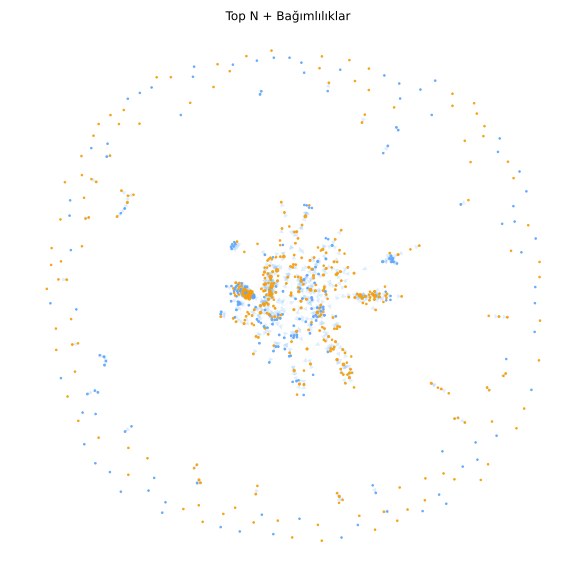
\includegraphics[width=\linewidth]{network_full_topN.png}
\caption{Top 1000 paket ağının görselleştirmesi. Yoğun bölgeler, ekosistemin omurgasını oluşturan alt kümeleri işaret etmektedir.}
\label{fig:network}
\end{figure}

\begin{figure}[H]
\centering
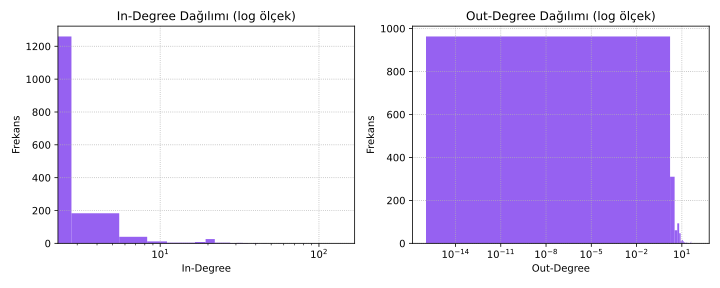
\includegraphics[width=\linewidth]{degree_histograms.png}
\caption{In-degree ve out-degree histogramları. Dağılımın ağır kuyruklu (heavy-tailed) yapısı, merkeziyetin az sayıda pakette toplandığını doğrulamaktadır.}
\label{fig:histograms}
\end{figure}

Şekil \ref{fig:network} ile sunulan ağ topolojisi, homojen bir dağılımdan ziyade, belirli çekim merkezleri etrafında yoğunlaşan belirgin bir kümelenme (clustering) eğilimi sergilemektedir. Derece dağılımlarının irdelendiği Şekil \ref{fig:histograms}, bu yapısal karakteristiği istatistiksel olarak doğrulamaktadır: Ağ, düğümlerin büyük çoğunluğunun marjinal sayıda bağlantıya sahip olduğu, buna karşın "hub" niteliğindeki elit bir azınlığın yüzlerce bağlantıyı domine ettiği, tipik bir "ölçekten bağımsız" (scale-free) mimari arz etmektedir. Dağılımın bu ağır kuyruklu (heavy-tailed) doğası, merkeziyetin ve dolayısıyla sistemik riskin, ekosistemin çok küçük bir fraksiyonunun tekelinde toplandığını kanıtlamaktadır.

\subsection{Merkeziyet İlişkileri}
\begin{figure}[H]
\centering
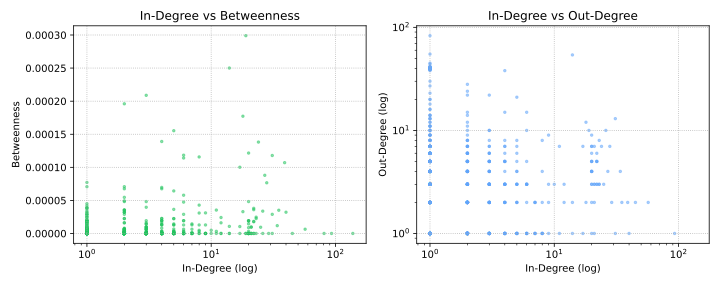
\includegraphics[width=\linewidth]{scatter_correlations.png}
\caption{Merkeziyet ölçüleri arasındaki korelasyonlar.}
\label{fig:scatter}
\end{figure}

Merkeziyet metrikleri arasındaki korelasyon matrisi (Şekil \ref{fig:scatter}), in-degree ile betweenness arasında pozitif yönlü ancak asimetrik bir ilişkiyi açığa çıkarmaktadır. Bu bulgu, yüksek popülariteye (in-degree) sahip olmayan bazı paketlerin, ağın izole kümelerini birbirine bağlayan kritik köprüler (yüksek betweenness) olarak stratejik bir rol üstlenebildiğini göstermektedir. Dolayısıyla, odağını yalnızca indirme sayılarına veya doğrudan bağımlılıklara kilitleyen geleneksel analizler, bu tür "gizli" yapısal darboğazları gözden kaçırma riskiyle maluldür.

\subsection{Kritik Düğümlerin Analizi}
\begin{table}[H]
\centering
\caption{\textsc{Top 10 In-Degree}}
\label{tab:indegree}
\resizebox{\linewidth}{!}{%
\begin{tabular}{lrrrr}
\toprule
Paket & In-Degree & Out-Degree & Betweenness & TopN? \\
\midrule
@babel/helper-plugin-utils & 110 & 0 & 0.000000 & True \\
call-bound & 41 & 2 & 0.000283 & False \\
postcss-value-parser & 39 & 0 & 0.000000 & True \\
call-bind & 36 & 4 & 0.000000 & False \\
@types/node & 34 & 1 & 0.000067 & False \\
debug & 34 & 1 & 0.000100 & True \\
es-errors & 33 & 0 & 0.000000 & False \\
@babel/types & 32 & 2 & 0.000236 & True \\
define-properties & 29 & 3 & 0.000000 & False \\
chalk & 28 & 0 & 0.000000 & False \\
\bottomrule
\end{tabular}%
}
\end{table}

\begin{table}[H]
\centering
\caption{\textsc{Top 10 Out-Degree}}
\label{tab:outdegree}
\resizebox{\linewidth}{!}{%
\begin{tabular}{lrrrr}
\toprule
Paket & Out-Degree & In-Degree & Betweenness & TopN? \\
\midrule
@babel/preset-env & 70 & 3 & 0.000000 & True \\
postcss-preset-env & 67 & 1 & 0.000000 & True \\
es-abstract & 54 & 17 & 0.000000 & False \\
react-scripts & 48 & 0 & 0.000000 & True \\
workbox-build & 37 & 1 & 0.000000 & True \\
eslint & 34 & 1 & 0.000000 & True \\
cssnano-preset-default & 30 & 1 & 0.000000 & True \\
webpack-dev-server & 28 & 1 & 0.000000 & True \\
@jest/core & 28 & 2 & 0.000000 & True \\
express & 27 & 1 & 0.000000 & True \\
\bottomrule
\end{tabular}%
}
\end{table}

\begin{table}[H]
\centering
\caption{\textsc{Top 10 Betweenness}}
\label{tab:betweenness}
\resizebox{\linewidth}{!}{%
\begin{tabular}{lrrrr}
\toprule
Paket & Betweenness & In-Degree & Out-Degree & TopN? \\
\midrule
jest-circus & 0.001144 & 1 & 20 & False \\
@babel/core & 0.001112 & 12 & 15 & True \\
babel-jest & 0.001087 & 2 & 7 & True \\
jest-runner & 0.001000 & 2 & 22 & True \\
@babel/helper-create-class-features-plugin & 0.000798 & 10 & 7 & True \\
get-intrinsic & 0.000771 & 22 & 10 & True \\
jest-snapshot & 0.000549 & 6 & 21 & True \\
@babel/traverse & 0.000523 & 20 & 7 & True \\
babel-preset-current-node-syntax & 0.000499 & 2 & 15 & False \\
babel-plugin-istanbul & 0.000466 & 2 & 5 & True \\
\bottomrule
\end{tabular}%
}
\end{table}
Merkeziyet metriklerine dayalı hiyerarşik sıralamalar, ekosistemdeki risk profillerinin çok katmanlı yapısını gözler önüne sermektedir. Tablo \ref{tab:indegree}'de listelenen ve in-degree zirvesini tutan paketler, ekosistemin en popüler ve güven duyulan yapı taşlarını temsil etmektedir. Öte yandan, Tablo \ref{tab:outdegree}'de öne çıkan \texttt{@babel/preset-env} gibi paketler, sahip oldukları yoğun dış bağımlılıklar nedeniyle geniş bir saldırı yüzeyi sunmakta ve tedarik zincirinin alt katmanlarından sızabilecek tehditlere karşı kırılgan bir profil çizmektedir. Tablo \ref{tab:betweenness} ise, popülerlikten bağımsız olarak, ağdaki bilgi ve risk trafiğini yöneten \texttt{jest-circus} gibi stratejik darboğazları ifşa etmektedir. Bu üç farklı perspektif, tek boyutlu analizlerin riskin bütüncül resmini çizmekte yetersiz kalacağını kanıtlar niteliktedir.

\subsection{Bileşik Risk Skoru (BRS) Sıralaması}
\begin{figure}[H]
\centering
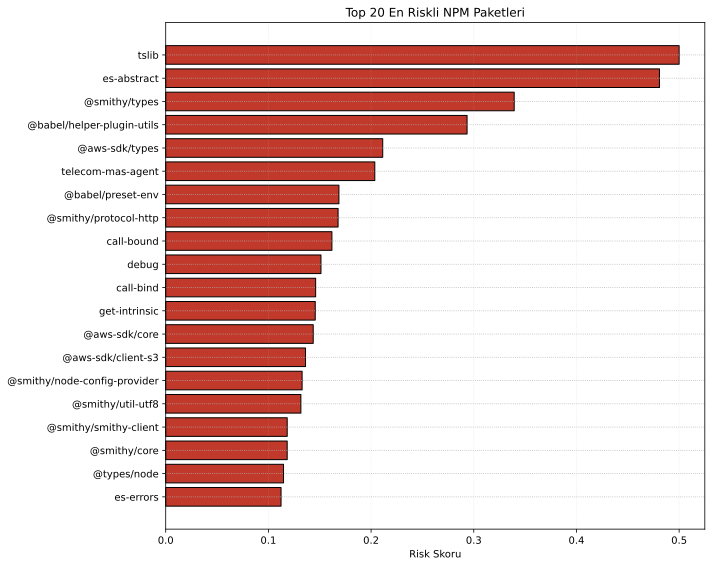
\includegraphics[width=\linewidth]{top20_risk_scores.png}
\caption{En yüksek Bileşik Risk Skoruna (BRS) sahip 20 paket.}
\label{fig:risk_scores}
\end{figure}

\begin{table}[H]
\centering
\caption{\textsc{Top 20 Bileşik Risk Skoru (BRS)}}
\label{tab:risk}
\resizebox{\linewidth}{!}{%
\begin{tabular}{lrrrrr}
\toprule
Paket & Risk & In-Degree & Out-Degree & Betweenness & TopN? \\
\midrule
@babel/helper-plugin-utils & 0.500000 & 110 & 0 & 0.000000 & True \\
@babel/core & 0.388827 & 12 & 15 & 0.001112 & True \\
jest-circus & 0.361688 & 1 & 20 & 0.001144 & False \\
jest-runner & 0.334157 & 2 & 22 & 0.001000 & True \\
get-intrinsic & 0.330606 & 22 & 10 & 0.000771 & True \\
babel-jest & 0.313975 & 2 & 7 & 0.001087 & True \\
@babel/helper-create-class-features-plugin & 0.274757 & 10 & 7 & 0.000798 & True \\
call-bound & 0.266206 & 41 & 2 & 0.000283 & False \\
@babel/traverse & 0.248118 & 20 & 7 & 0.000523 & True \\
es-abstract & 0.231558 & 17 & 54 & 0.000000 & False \\
jest-snapshot & 0.231168 & 6 & 21 & 0.000549 & True \\
@babel/preset-env & 0.213636 & 3 & 70 & 0.000000 & True \\
@babel/types & 0.212942 & 32 & 2 & 0.000236 & True \\
postcss-preset-env & 0.195974 & 1 & 67 & 0.000000 & True \\
@jest/types & 0.193414 & 26 & 7 & 0.000211 & True \\
debug & 0.183565 & 34 & 1 & 0.000100 & True \\
babel-preset-current-node-syntax & 0.182762 & 2 & 15 & 0.000499 & False \\
postcss-value-parser & 0.177273 & 39 & 0 & 0.000000 & True \\
call-bind & 0.175065 & 36 & 4 & 0.000000 & False \\
@types/node & 0.174844 & 34 & 1 & 0.000067 & False \\
\bottomrule
\end{tabular}%
}
\end{table}
Önerilen BRS modeli, popülerlik, saldırı yüzeyi ve stratejik konumlanma gibi üç farklı risk boyutunu tek bir potada eriterek, tekil metriklerin yakalayamadığı hibrit risk profillerini görünür kılmaktadır. Şekil \ref{fig:risk_scores} ve Tablo \ref{tab:risk}'te izlendiği üzere, \texttt{@babel/core} ve \texttt{jest-runner} gibi paketler, hem yüksek popülariteleri hem de ağdaki stratejik konumları sebebiyle risk sıralamasının zirvesine yerleşmektedir. Bu hiyerarşi, güvenlik denetimleri ve kaynak tahsisinde önceliklendirilmesi elzem olan "yüksek değerli hedefleri" (high-value targets) tartışmaya yer bırakmayacak netlikte tanımlamaktadır.

\subsection{Sistemik Etki ve Kaskad Analizi}
\begin{figure}[H]
\centering
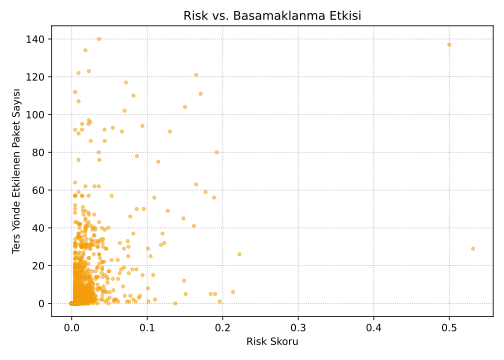
\includegraphics[width=\linewidth]{risk_vs_cascade.png}
\caption{BRS ile kaskad etki (erişilebilirlik) arasındaki ilişki.}
\label{fig:cascade}
\end{figure}

\begin{figure}[H]
\centering
\includegraphics[width=\linewidth]{top20_cascade_impact.png}
\caption{İlk 20 paketin çıkarılmasının LCC ve erişilebilirlik üzerindeki yıkıcı etkisi.}
\label{fig:impact}
\end{figure}
BRS metriğinin öngörü gücünü sınayan hedefli saldırı simülasyonları, modelin geçerliliğini çarpıcı bir biçimde ortaya koymaktadır. Şekil \ref{fig:impact}'te görüldüğü üzere, BRS zirvesindeki paketlerin ağdan koparılması, rastgele düğüm seçimine kıyasla En Büyük Bağlı Bileşen (LCC) boyutunda çok daha yıkıcı bir çöküşe neden olmakta ve ağın bütünlüğünü hızla parçalamaktadır. BRS skoru ile kaskad etki (bir düğümün kaybından etkilenen toplam paket sayısı) arasındaki güçlü pozitif korelasyon (Şekil \ref{fig:cascade}) da bu tespiti perçinlemektedir. Bu veriler, BRS'nin yalnızca statik bir kritiklik ölçütü olmadığını, aynı zamanda bir düğümün ele geçirilmesinin tüm ekosistemde tetikleyebileceği zincirleme reaksiyonun da güvenilir bir habercisi olduğunu teyit etmektedir.

\section{Tartışma ve Sonuç}
Bu çalışma, NPM ekosistemindeki sistemik riski, paket içeriğinden bağımsız olarak salt topolojik parametreler üzerinden modelleyen BRS (Bileşik Risk Skoru) metodolojisini literatüre kazandırmış ve geçerliliğini ampirik olarak kanıtlamıştır. Yürütülen analizler, ekosistem güvenliğinin, tehlikeye girmeleri halinde domino etkisiyle ağın bütünlüğünü çökertme potansiyeli taşıyan az sayıda "omurga" paketin sırtında yükseldiğini nicel verilerle doğrulamıştır.

Elde edilen bulgular ve önerilen model, teorik bir egzersiz olmanın ötesine geçerek, yazılım tedarik zinciri güvenliğini operasyonel düzeyde tahkim edecek somut stratejiler sunmaktadır:
\begin{itemize}
    \item \textbf{Tespit Hatlarında Önceliklendirme:} Amalfi ve Cerebro gibi savunma mekanizmalarında tarama kaynaklarının, BRS skoru yüksek paketlere kanalize edilerek verimliliğin artırılması.
    \item \textbf{Politika Geliştirme:} in-toto \cite{lit13} gibi katı güvenlik protokollerinin, SBOM (Yazılım Malzeme Listesi) uygulamalarının \cite{lit3, lit9} ve dijital imza/bütünlük kontrollerinin \cite{lit21, lit26, lit27} öncelikle bu çalışmada saptanan kritik düğümlere uygulanarak riskin kaynağında boğulması.
    \item \textbf{Bakımcı Farkındalığı:} Kritik paket sahiplerine risk skorlarının bildirilmesi yoluyla, iki faktörlü kimlik doğrulama (2FA) ve daha titiz kod inceleme pratiklerinin benimsenmesinin teşvik edilmesi.
\end{itemize}

Gelecek çalışmalara yönelik öneriler, geliştirilen modeli paketler arasındaki teknik bağların ötesine taşıyarak, geliştirici ağları (maintainer networks) ve sosyal bağımlılıklar gibi insan faktörlerini de kapsayacak şekilde genişletmektir. Ayrıca, ekosistemin zamana bağlı dinamiklerini mercek altına alan boylamsal (temporal) bir yaklaşım, riskin evrimini ve dönüşümünü anlamlandırmak adına paha biçilmez bir perspektif sunacaktır.

\section{Yen{\footnotesize İ}den Üret{\footnotesize İ}leb{\footnotesize İ}rl{\footnotesize İ}k}
Çalışmanın şeffaflığını ve tekrarlanabilirliğini sağlamak adına tüm kaynak kodlar ve veri setleri erişime açıktır:
\begin{itemize}
  \item \textbf{Analiz Kodları:} \texttt{analysis/analysis.ipynb} (Python 3, NetworkX, pandas).
  \item \textbf{Veri Çıktıları:} Tüm ara sonuçlar ve metrikler \texttt{results/} dizininde CSV/JSON formatında sunulmuştur.
\end{itemize}

% APA-style bibliography 
\begin{thebibliography}{30}

\bibitem{lit1} E. Wyss, ``A new frontier for software security: Diving deep into npm,'' 2025.

\bibitem{lit7} M. Wang, P. Wu, and Q. Luo, ``Construction of software supply chain threat portrait based on chain perspective,'' 2023.

\bibitem{lit8} C. Liu et al., ``Demystifying vulnerability propagation via dependency trees in npm,'' in \textit{ICSE}, 2022.

\bibitem{lit18} A. Zerouali et al., ``On the impact of security vulnerabilities in the npm and RubyGems dependency networks,'' 2022.

\bibitem{lit5} I. Rahman et al., ``Characterizing dependency update practice of NPM, PyPI and Cargo packages,'' 2024.

\bibitem{lit22} F. R. Cogo, ``Studying dependency maintenance practices through mining NPM,'' 2020.

\bibitem{lit10} A. J. Jafari et al., ``Dependency practices for vulnerability mitigation,'' 2023.

\bibitem{lit20} M. Zimmermann et al., ``Small world with high risks: Security threats in npm,'' in \textit{USENIX Sec.}, 2019.

\bibitem{lit16} A. Hafner, A. Mur, and J. Bernard, ``Node package manager's dependency network robustness,'' 2021.

\bibitem{lit25} E.-R. Oldnall, ``The web of dependencies: A complex network analysis of the NPM,'' 2017.

\bibitem{lit2} P. Jaisri, B. Reid, and R. G. Kula, ``A preliminary study on self-contained libraries in the NPM ecosystem,'' 2024.

\bibitem{lit6} T. G. Hastings, ``Combating source poisoning and next-generation software supply chain attacks,'' 2024.

\bibitem{lit30} M. Shcherbakov, P. Moosbrugger, and M. Balliu, ``Unveiling the invisible: Prototype pollution gadgets via dynamic taint,'' 2021.

\bibitem{lit12} D. Y. K. Yip, ``Empirical study on dependency-based attacks in Node.js,'' 2022.

\bibitem{lit4} M. Ohm et al., ``Backstabber's knife collection: A review of open source software supply chain attacks,'' in \textit{DIMVA}, 2020.

\bibitem{lit24} P. Ladisa et al., ``The hitchhiker's guide to malicious third-party dependencies,'' in \textit{IEEE S\&P}, 2023.

\bibitem{lit28} R. Duan et al., ``Towards measuring supply chain attacks on package managers,'' in \textit{NDSS}, 2020.

\bibitem{lit19} A. Sejfia and M. Schafer, ``Practical automated detection of malicious npm packages (Amalfi),'' in \textit{ICSE}, 2022.

\bibitem{lit29} X. Zheng et al., ``Towards robust detection of OSS supply chain poisoning (OSCAR),'' 2024.

\bibitem{lit15} S. Halder et al., ``Malicious package detection using metadata information,'' 2024.

\bibitem{lit14} J. Zhang et al., ``Malicious package detection in NPM and PyPI using a single model of malicious behavior sequence,'' 2023.

\bibitem{lit17} P. Ladisa et al., ``On the feasibility of cross-language detection of malicious packages in npm and PyPI,'' 2023.

\bibitem{lit11} M. L. P. Correia, ``Detection of software supply chain attacks in code repositories,'' 2022.

\bibitem{lit23} M. Ohm et al., ``Supporting detection via unsupervised signature generation (ACME),'' 2021.

\bibitem{lit13} S. Torres-Arias, ``In-toto: Practical software supply chain security,'' in \textit{USENIX Sec.}, 2020.

\bibitem{lit3} S. Yu, ``Accurate and efficient SBOM generation for software supply chain security,'' 2024.

\bibitem{lit9} H. E. Ahlstrom, ``Dependency analysis for software licensing and security,'' 2025.

\bibitem{lit21} T. R. Schorlemmer, ``Software supply chain security: Attacks, defenses, and signing adoption,'' 2024.

\bibitem{lit26} N. Imtiaz, ``Toward secure use of open source dependencies,'' 2023.

\bibitem{lit27} S. Vaidya, ``Towards ensuring integrity and authenticity of software repositories,'' 2022.

\end{thebibliography}


\end{document}
